This chapter provides discussion of load balancer suitable for container clusters.
First the author discusses problems of conventions architecture in Section~\ref{problem_k8s}.
Then the author proposes the best one in Section~\ref{proposed_arch}.
After that the author discusses inplementation of  a portable and redundant load balancer in Section~\ref{portable_lb}. 

This chapter presents implementation of the proof of the concept system for the proposed load balancer architecture in detail.
First overall architecure is explained in Section~\ref{sec:poc}.
Then ipvs containerization is explained in detail in Section~\ref{sec:ipvs}.
Finally implementation of BGP software container is explained in Section~\ref{sec:bgp}.

\section{Architecture}

\subsection{Problem of Conventional Architecture}\label{problem_k8s}

\begin{figure}[tb]

  \begin{subfigure}[t]{\columnwidth}
    \centering
    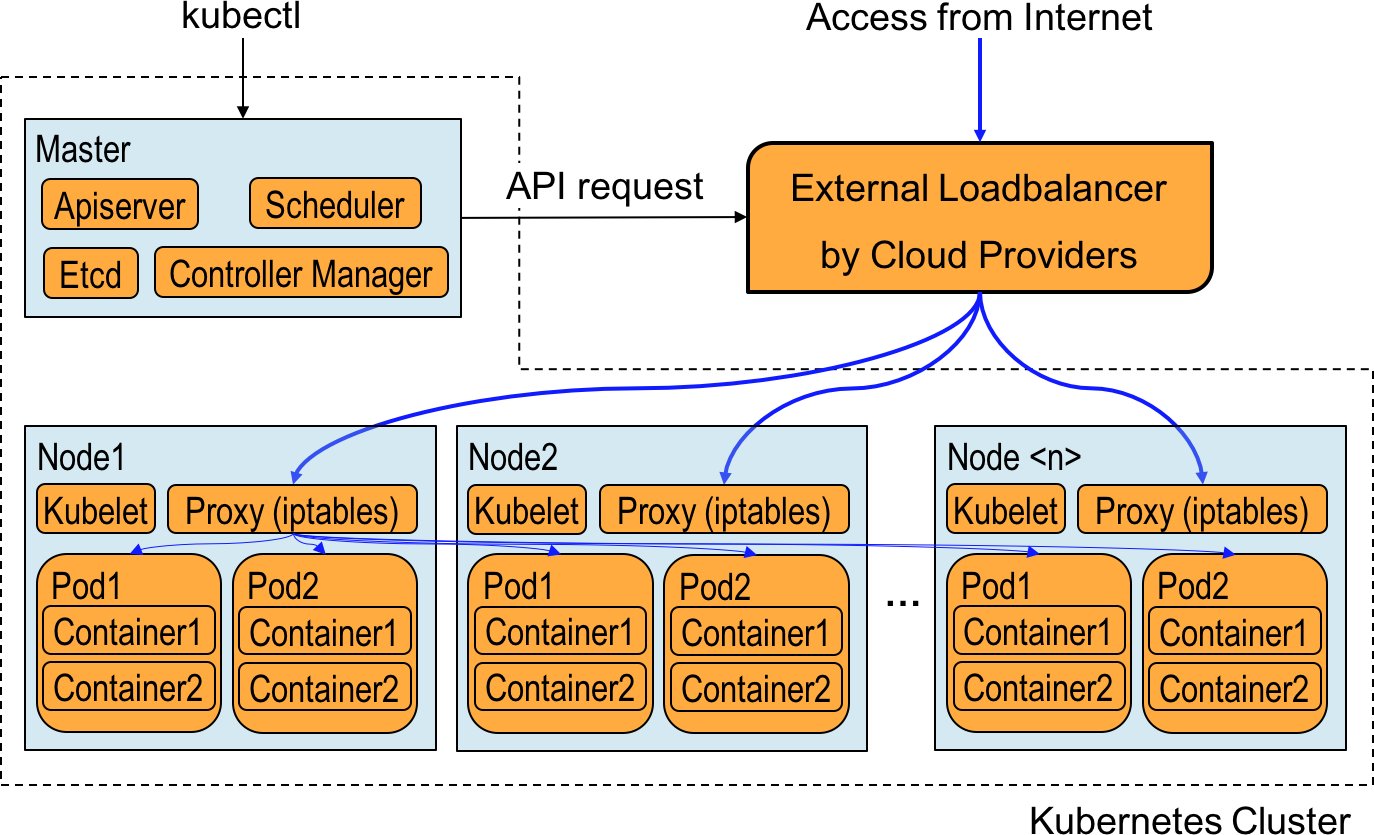
\includegraphics[width=0.8\columnwidth]{Figs/K8sConventional}
    \caption{Kubernetes in cloud infrastructures}
    \label{fig:K8sConventional}
  \end{subfigure}

  \par\bigskip
  \par\bigskip

  \begin{subfigure}[t]{\columnwidth}
    \centering
    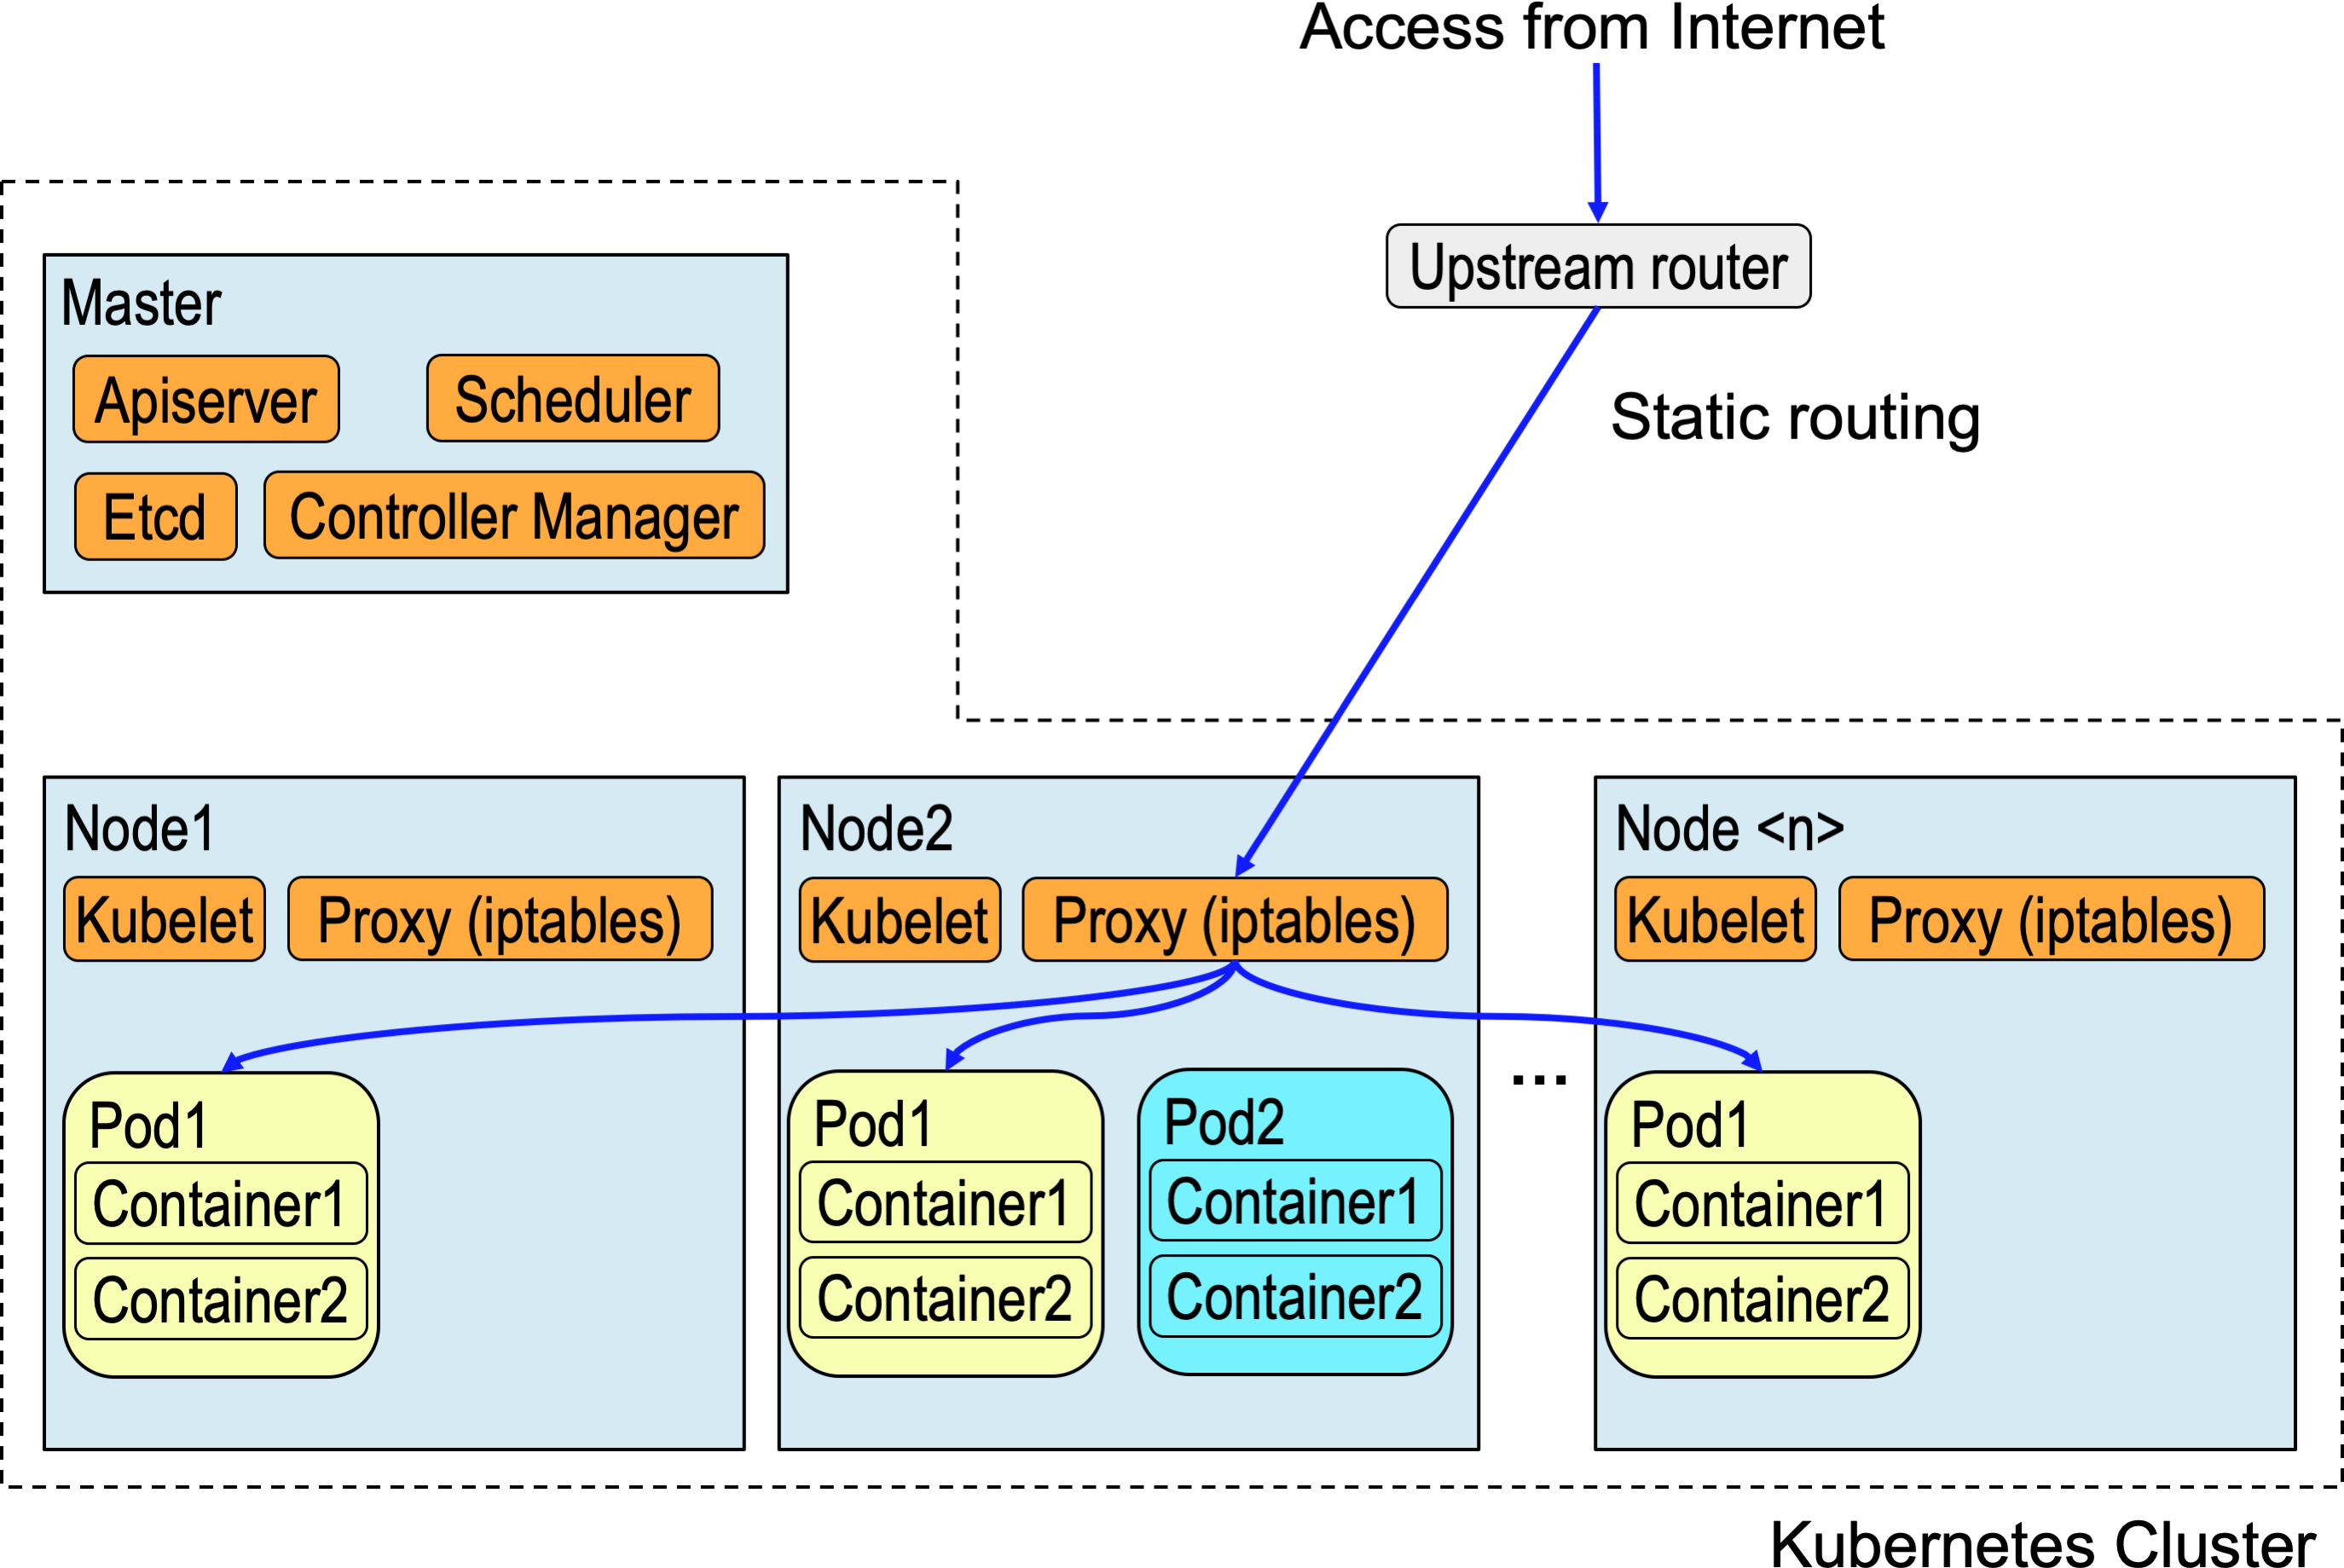
\includegraphics[width=0.8\columnwidth]{Figs/K8sConventional_bm}
    \caption{Kubernetes in on-premise data centers}
    \label{fig:K8sConventional_bm}
  \end{subfigure}

  \caption{Conventional architecture of a Kubernetes cluster}
  
  \centering
  \begin{minipage}{0.9\columnwidth}
    In supported infrastructures, e.g., major cloud providers, Kubernetes automatically set up route to the service IPs, when web service providers launch  container clusters.
    In unsupported infrastructures, e.g., on-premise data centers, they have to manually set up the route. 
  \end{minipage}

%  \label{fig:exabgp}
\end{figure}

The problem of Kubernetes is its partial support for the ingress traffic routing.
Figure~\ref{fig:K8sConventional} shows an exemplified Kubernetes cluster.
A Kubernetes cluster typically consists of a master and nodes. They can be physical servers or VMs.
On the master, daemons that control the Kubernetes cluster are typically deployed. 
These daemons include, apiserver, scheduler, controller-manager and etcd. 
On the nodes, kubelet and proxy are deployed.
The kubelet daemon will run {\it pods}, depending on the PodSpec information obtained from the apiserver on the master.
The proxy daemon will set up iptables DNAT rules that function as the internal load balancer.
A {\em pod} is a group of containers that share the same network namespace and cgroup,
and is the basic execution unit in a Kubernetes cluster.

When a service is created, the master schedules where to run {\em pods} and kubelets on the nodes launch them accordingly.
At the same time, the master sends out requests to cloud provider's API endpoints, asking them to set up external cloud load balancers that distribute ingress traffic to every node in the Kubernetes cluster.
The proxy daemon on the nodes also setup iptables DNAT\cite{MartinA.Brown2017} rules. 
The Ingress traffic will then be evenly distributed by the cloud load balancer to nodes, 
after which it will be distributed again by the DNAT rules on the nodes to the designated {\em pods}. 
The returning packets follows the exact same route as the incoming ones.

This architecture has the followings problems: 
1) There must exist cloud load balancers whose APIs are supported by the Kubernetes daemons.
There are numerous load balancers which is not supported by the Kubernetes.
These include the bare metal load balancers for on-premise data centers.
2) Distributing the traffic twice, first on the external load balancers and second on each node, complicates the administration of packet routing. 
Imagine a situation in which the DNAT table on one of the nodes malfunctions.
In such a case, only occasional timeouts would be observed, and hence it would be very difficult to find out which node is malfunctioning.   

Regarding the first problem, if there is no load balancer that is not supported by Kubernetes, users must manually set up the static route on the upstream router, every time they launch the web application clusters, as is shown in Figure~\ref{fig:K8sConventional_bm}.
The traffic would be routed to a node then distributed by the DNAT rules on the node to the designated {\em pods}.
However, in the cases where the upstream router is administered by different organizations, users are always required to negotiate with them about adding a route to their new application cluster.
Therefore this approach significantly degrades the portability of container clusters.
Furthermore, a static route usually lacks redundancy and scalability.

In short, 1) while Kubernetes is effective in major cloud providers, it fails to provide portability for container clusters in environments where there is no supported load balancer, and 2) the routes incoming traffic follow are very complex.
In order to address these problems, the author proposes a containerized software load balancer 
that is deployable in any environment even if there are no external load balancers.

\FloatBarrier

%\section{Proposed Load Balancer}\label{proposed_arch}
\subsection{Load balancer in container}

The author proposes a load balancer architecture, where a cluster of load balancers are deployed as containers.
Figure~\ref{fig:K8sProposed} shows the proposed load balancer architecture for Kubernetes,
which has the following characteristics;
1) Each load balancer itself is run as a {\em pod} by Kubernetes. 
2) Load balancing tables are dynamically updated based on information about running {\em pods}.
3) There exist multiple load balancers for redundancy and scalability.
4) The routing table in the upstream router are updated dynamically using standard network protocol.

\begin{figure}[h]
  \centering
  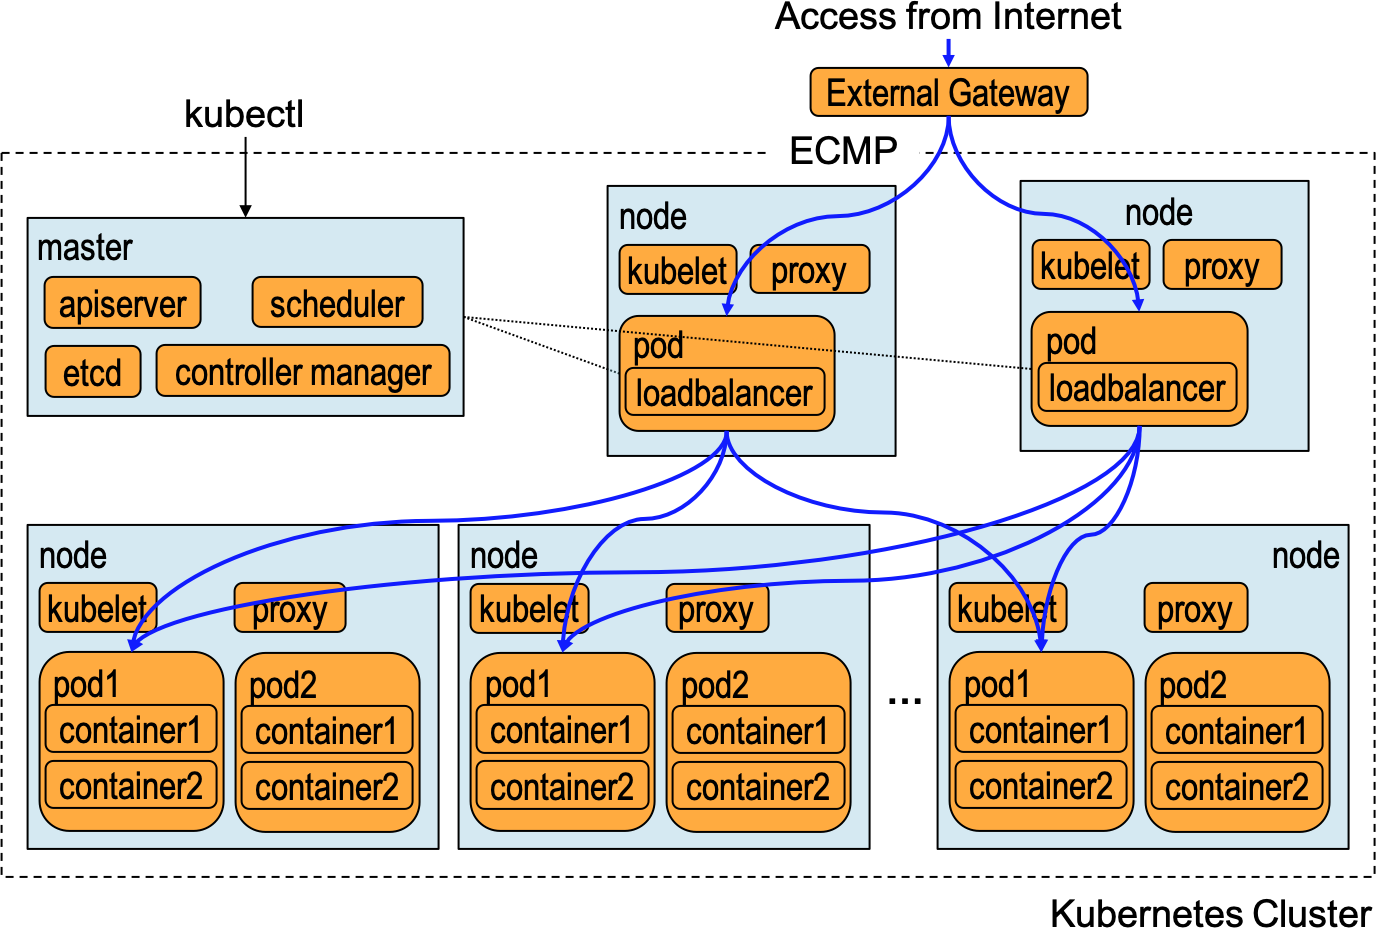
\includegraphics[width=0.8\columnwidth]{Figs/K8sProposed}
  \caption{Kubernetes cluster with proposed load balancer.}
  \label{fig:K8sProposed}
\end{figure}

The proposed load balancer can resolve the conventional architecture problems.
Since the load balancer itself is containerized, the load balancer can run in any environment including on-premise data centers,
even without external load balancers that is supported by Kubernetes.
The incoming traffic is directly distributed to designated {\em pods} by the load balancer.
It makes the administration, e.g. finding malfunctions, easier.

Furthermore, the proposed load balancer has other benefits.
Since a software load balancer in a container can run on any Linux system, it can share the server pool with web containers.
Users can utilize existing servers rather than buying dedicated hardware.

Because a cluster of load balancer containers is controlled by Kubernetes, it becomes redundant and scalable.
Kubernetes always tries to maintain the number of load balancer containers at the number specified by the user.
If a single container fails, Kubernetes schedule and launch another one on a different node, which provides the resilience to failures.
When there is a huge spike in the traffic, it can quickly scale the size of the cluster depending on the demand.

The routes to the load balancers are automatically updated through the standard protocol, BGP.
Therefore users do not need to manually add the route every time new load balancer container is launched, as is the case in the conventional architecture.

\FloatBarrier

\subsection{Redundancy with ECMP}

\begin{figure}[tb]
  \centering
  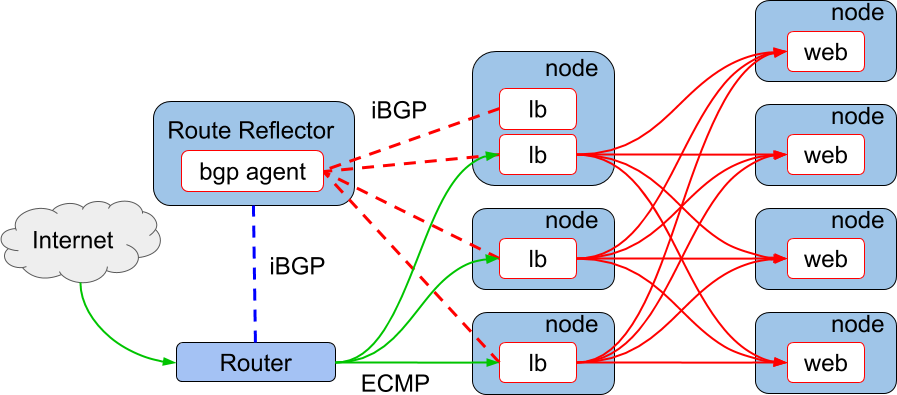
\includegraphics[width=0.8\columnwidth]{Figs/ecmp.png}
\caption{The proposed architecture of load balancer redundancy with ECMP.}

\vspace{1mm}

\begin{minipage}{0.9\columnwidth}
%\small\raggedright
  The traffic from the internet is distributed by the upstream router to multiple of lb pods using hash-based ECMP and then distributed by the lb pods to web pods using Linux kernel's ipvs.
  The ECMP routing table on the upstream router is populated using iBGP.
\end{minipage}
\label{fig:ecmp}
\end{figure}

Fig.~\ref{fig:ecmp} shows a schematic diagram to explain redundancy architecture with Equal Cost Multi Path(ECMP) for the proposed load balancer.
%
The ECMP is a functionality a router supports, where the router has multiple next hops with equal priority(cost) to a destination.
And the router generally distributes the traffic to the multiple next hops depending on the hash of five-tuples(source IP, destination IP, source port, destination port, protocol) of the flow.
The multiple next hops and their cost are often populated using the BGP protocol.
%
The notable benefit of the ECMP setup is its scalability.
All the load balancers that claims as the next hop is active, i.e., all of them are utilized to increase the performance level.
Since the traffic from the internet is distributed by the upstream router, the overall throughput is limited by performance levels of the router after all.
However, in practice, there are a lot of cases where this architecture is beneficial.
For example, if a software load balancer is capable of handling 1 Gbps equivalent of traffic and the upstream router is capable of handling 10 Gbps, it still is worthwhile launching 10 of the software load balancer containers to fill up maximum throughput of the upstream router.

%
In the proposed redundant architecture, there exists a node with the knowledge of the overlay network as a route reflector
A route reflector is a network component for BGP to reduce the number of peerings by aggregating the routing information\cite{rfc4456}.
In the proposed architecture the author uses it as a delegater for load balancer containers towards the upstream router.

The route reflector exists for a practical reason, i.e, to deal with the complexity due to the overlay network.
Since the upstream router normally has no knowledge of the overlay network and IP addresses used inside the Kubernetes clusters, a container must rely on SNAT on the node to communicate with the router.
The SNAT caused a problem when the author tried a set up without the route reflector, to co-host multiple load balancer containers for different services on a single node.
Because of the SNAT, the source IP addresses of multiple connections were translated into the node IP address.
The BGP agent on the router was confused by these connections and cloud not properly set up ECMP route for separate services.
This was due to the fact that the BGP agent used in the experiment used only the source IP address of the connection to distinguish the BGP peer.

In addition to that the route reflector brings another benefit. 
The upstream router does not need to accept BGP sessions from containers with random IP addresses, but only from the route reflector with well known fixed IP address. 
This is preferable in terms of security especially when a different organization administers the upstream router.

By using the route reflector, we can have the following benefits.
1) Each node can accommodate multiple load balancer containers. This was not possible when we tried to directly connect load balancers and the router through SNAT.
2) The router does not need to allow peering connections from random IP addresses that may be used by load balancer containers. Now, the router only need to have the reflector information as the BGP peer definition.

Since we use standard Linux boxes for route reflectors, we can configure them as we like;
a) We can make them belong to overlay network so that multiple BGP sessions from a single node can be established.
b) We can use a BGP agent that supports dynamic neighbor (or dynamic peer), where one only needs to define the IP range as a peer group and does away with specifying every possible IP that load balancers may use.
Although not shown in the Fig.~\ref{fig:ecmp}, we could also place another route reflector for redundancy purpose.

%\section{Proof of concept system}\label{sec:poc}

\FloatBarrier


